
%(BEGIN_QUESTION)
% Copyright 2007, Tony R. Kuphaldt, released under the Creative Commons Attribution License (v 1.0)
% This means you may do almost anything with this work of mine, so long as you give me proper credit

One way to decrease the amount of energy consumed in the pumping of liquids is to use a variable-speed electric motor to turn the pump instead of turning the pump full speed and throttling with a control valve:

$$\includegraphics[width=15.5cm]{i01783x01.eps}$$

A significant advantage to using a control valve to regulate liquid flow is faster speed of response.  If the process requires fast flow-control response, there may be no option but to use a control valve to throttle flow, which will inevitably waste energy.  We may realize the best of both worlds by using this hybrid control strategy:

$$\includegraphics[width=15.5cm]{i01783x02.eps}$$

The ZIC (Position Indicating Controller) varies the pump motor speed to achieve a particular stem position on the control valve.  The local setpoint (LSP) for this position controller is usually set $>$75\%.  Explain how this system works to conserve energy, and also which direction of action each controller must have (direct or reverse).

\vskip 20pt \vbox{\hrule \hbox{\strut \vrule{} {\bf Suggestions for Socratic discussion} \vrule} \hrule}

\begin{itemize}
\item{} A useful analytical technique for any complex control system is to annotate the diagram with ``+'' and ``$-$'' symbols at the instrument bubble inputs, designating ``noninverting'' and ``inverting'' characteristics, respectively.  Show how this helps you track of all directions of action, making it easier to figure out how the control system responds to changes.
\item{} For those who have studied PID control, explain why one of these two controllers (FIC or ZIC) needs to be tuned much faster than the other to avoid instability.  Identify the controller which needs to be ``faster,'' (more aggressive integral action), and explain why.
\end{itemize}


\underbar{file i01783}
%(END_QUESTION)





%(BEGIN_ANSWER)

$$\includegraphics[width=15.5cm]{i01783x03.eps}$$

If the flow rate suddenly increases due to some load, the control valve will immediately pinch down to bring the flow back to setpoint.  However, the position controller will notice the new (lower) valve position and slowly turn down the pump's speed to allow the control valve to open back up to its former position where it is less restrictive and therefore wastes less pumping energy.

\vskip 10pt

If the flow rate suddenly decreases due to some load, the control valve will immediately open up to bring the flow back to setpoint.  However, the position controller will notice the new (higher) valve position and slowly turn up the pump's speed to allow the control valve to close back down to its former position where it has more freedom of motion to control flow.

\vskip 10pt

It is bad to configure a controller for a faster response than its final control element is able to respond.  Since the electric motor is slower-responding than the control valve, the valve's controller must be tuned ``faster.''

%(END_ANSWER)





%(BEGIN_NOTES)


%INDEX% Control, strategies: valve position optimization

%(END_NOTES)


